\documentclass[tikz,border=10pt]{standalone}
\usetikzlibrary{positioning,arrows.meta,fit,backgrounds,shapes.symbols,calc}

\definecolor{coreindigo}{HTML}{3F51B5}
\definecolor{ifgreen}{HTML}{4CAF50}
\definecolor{adaptorange}{HTML}{FF9800}
\definecolor{syncpurple}{HTML}{9C27B0}
\definecolor{domteal}{HTML}{009688}
\definecolor{fsgray}{HTML}{757575}
\definecolor{lightindigo}{HTML}{E8EAF6}
\definecolor{lightgreen}{HTML}{E8F5E9}
\definecolor{lightorange}{HTML}{FFF3E0}
\definecolor{lightpurple}{HTML}{F3E5F5}
\definecolor{lightteal}{HTML}{E0F2F1}
\definecolor{lightgray}{HTML}{F5F5F5}

\begin{document}
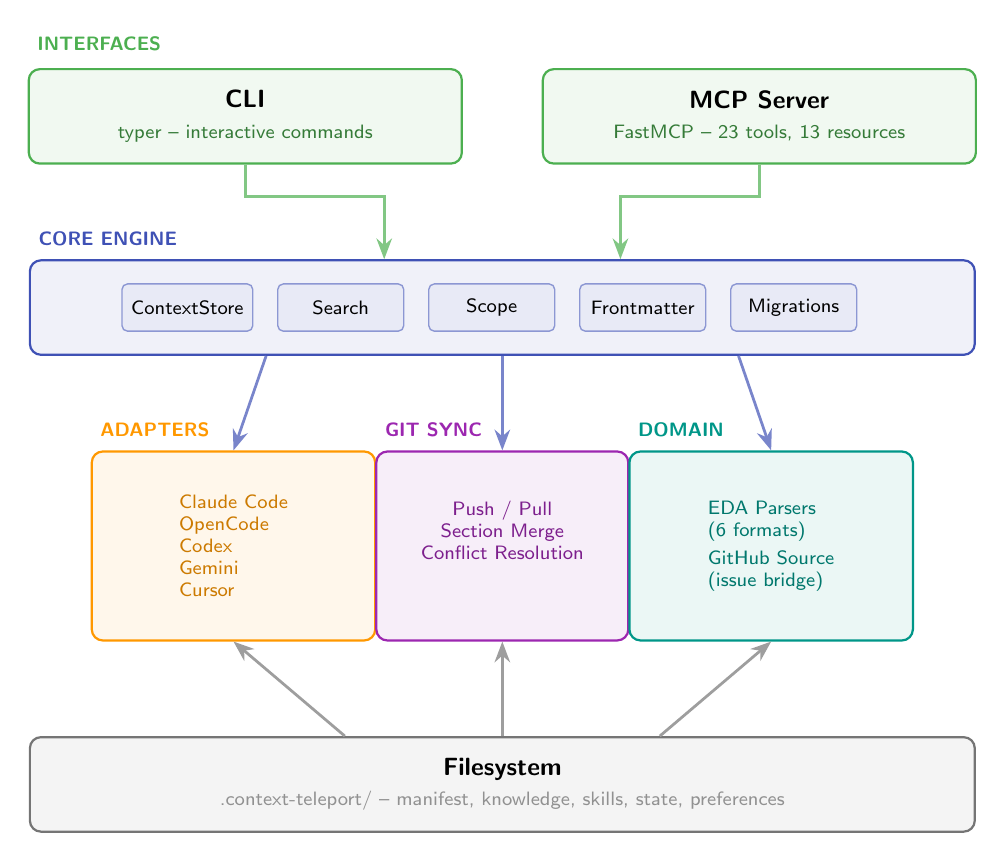
\begin{tikzpicture}[
    >=Stealth,
    every node/.style={font=\sffamily\small},
    box/.style={
        draw=#1, fill=#1!8, rounded corners=4pt,
        minimum width=4.8cm, minimum height=1.2cm,
        line width=0.8pt, align=center
    },
    innerbox/.style={
        draw=#1!60, fill=#1!12, rounded corners=2pt,
        minimum width=1.6cm, minimum height=0.6cm,
        line width=0.5pt, font=\sffamily\scriptsize, align=center
    },
    arr/.style={->, thick, color=#1!70, line width=1pt},
    label/.style={font=\sffamily\scriptsize\bfseries, color=#1},
]

% === Top Row: Interfaces ===
\node[box=ifgreen, minimum width=5.5cm] (cli)
    {\textbf{CLI}\\\textcolor{ifgreen!70!black}{\scriptsize typer -- interactive commands}};
\node[box=ifgreen, minimum width=5.5cm, right=1cm of cli] (mcp)
    {\textbf{MCP Server}\\\textcolor{ifgreen!70!black}{\scriptsize FastMCP -- 23 tools, 13 resources}};

% Interface label
\node[label=ifgreen, above=0.1cm of cli.north west, anchor=south west] {INTERFACES};

% === Middle Row: Core Engine ===
\node[box=coreindigo, minimum width=12cm, below=1.2cm of $(cli.south)!0.5!(mcp.south)$] (coreframe) {};

% Core inner components
\node[innerbox=coreindigo] at ([xshift=-4cm]coreframe.center) (store) {ContextStore};
\node[innerbox=coreindigo, right=0.3cm of store] (search) {Search};
\node[innerbox=coreindigo, right=0.3cm of search] (scope) {Scope};
\node[innerbox=coreindigo, right=0.3cm of scope] (front) {Frontmatter};
\node[innerbox=coreindigo, right=0.3cm of front] (migr) {Migrations};

% Core label
\node[label=coreindigo, above=0.05cm of coreframe.north west, anchor=south west] {\textbf{CORE ENGINE}};

% === Lower Row: Three Columns ===
% Left: Adapters
\node[box=adaptorange, minimum width=3.6cm, minimum height=2.4cm,
    below left=1.2cm and 1.6cm of coreframe.south] (adapters) {};
\node[label=adaptorange, above=0.05cm of adapters.north west, anchor=south west] {\textbf{ADAPTERS}};
\node[font=\sffamily\scriptsize, align=left, text=adaptorange!80!black] at (adapters.center) {
    Claude Code\\OpenCode\\Codex\\Gemini\\Cursor
};

% Center: GitSync
\node[box=syncpurple, minimum width=3.2cm, minimum height=2.4cm,
    below=1.2cm of coreframe.south] (gitsync) {};
\node[label=syncpurple, above=0.05cm of gitsync.north west, anchor=south west] {\textbf{GIT SYNC}};
\node[font=\sffamily\scriptsize, align=center, text=syncpurple!80!black] at ([yshift=0.2cm]gitsync.center) {
    Push / Pull\\Section Merge\\Conflict Resolution
};

% Git Remote cloud
\node[cloud, draw=syncpurple!60, fill=syncpurple!8, cloud puffs=10,
    cloud puff arc=120, minimum width=2.2cm, minimum height=1cm,
    right=0.8cm of gitsync, font=\sffamily\scriptsize\itshape, text=syncpurple!70!black]
    (remote) {Git Remote};
\draw[arr=syncpurple] (gitsync.east) -- (remote.west);

% Right: Domain Extensions
\node[box=domteal, minimum width=3.6cm, minimum height=2.4cm,
    below right=1.2cm and 1.6cm of coreframe.south] (domain) {};
\node[label=domteal, above=0.05cm of domain.north west, anchor=south west] {\textbf{DOMAIN}};
\node[font=\sffamily\scriptsize, align=left, text=domteal!80!black] at (domain.center) {
    EDA Parsers\\{\scriptsize (6 formats)}\\[2pt]GitHub Source\\{\scriptsize (issue bridge)}
};

% === Bottom: Filesystem ===
\node[box=fsgray, minimum width=12cm,
    below=1.2cm of gitsync.south] (fs) {
    \textbf{Filesystem}\\
    \textcolor{fsgray!80}{\scriptsize .context-teleport/ -- manifest, knowledge, skills, state, preferences}
};

% === Arrows ===
% Interfaces -> Core
\draw[arr=ifgreen] (cli.south) -- ++(0,-0.4) -| ([xshift=-1.5cm]coreframe.north);
\draw[arr=ifgreen] (mcp.south) -- ++(0,-0.4) -| ([xshift=1.5cm]coreframe.north);

% Core -> Lower row
\draw[arr=coreindigo] ([xshift=-3cm]coreframe.south) -- (adapters.north);
\draw[arr=coreindigo] (coreframe.south) -- (gitsync.north);
\draw[arr=coreindigo] ([xshift=3cm]coreframe.south) -- (domain.north);

% Core -> Filesystem
\draw[arr=fsgray] ([xshift=-2cm]fs.north) -- (adapters.south);
\draw[arr=fsgray] (fs.north) -- (gitsync.south);
\draw[arr=fsgray] ([xshift=2cm]fs.north) -- (domain.south);

\end{tikzpicture}
\end{document}
